\documentclass{amsart}
\usepackage[utf8]{inputenc}
\usepackage{graphicx}
\usepackage{enumerate}
\usepackage{comment}
\usepackage{multirow}
\usepackage[a4paper]{geometry}
\geometry{ a4paper, left = 1cm, right = 1cm, top = 1cm, bottom = 1cm}

\begin{document}
    \hrule
    \begin{center}
        \textbf{ Lamma    Tommaso    0000881007        Turno    II }\\
    \end{center}
    \hrule
    \begin{center}
        {\huge Misura della caratteristica di uscita di un BJT P-N-P \\ in configurazione a emettitore comune}
    \end{center}
    Nella prova si sono prese le caratteristiche in uscita alle correnti di base $100 \mu A$ e $200 \mu A$.
    Il circuito utilizzato per la prova è il seguente :
    \begin{center}
        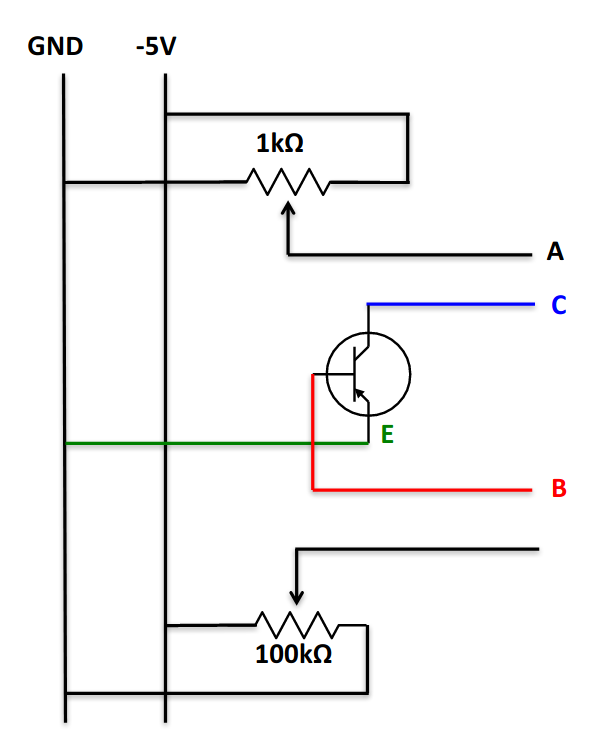
\includegraphics[width = 5cm, height = 7cm]{circuito.png}.
    \end{center}
    Gli strumenti utilizzati nella prova sono:
    \begin{enumerate}[(i)]
        \item Potenziometro da 1$k\Omega$
        \item Potenziometro da 100$k\Omega$
        \item Transistor BJT 2N3906(BU) (Si PNP) 
        \item Breadboard generica
        \item Oscilloscopio GOS-652 GW
        \item Multimetro digitale FLUKE 77
        \item Generatore di tensione continua IPS 3303 ISO-TECH
    \end{enumerate}
    \hfill \\
    I grafici delle caratteristiche in uscita sono:\\
    \begin{center}
        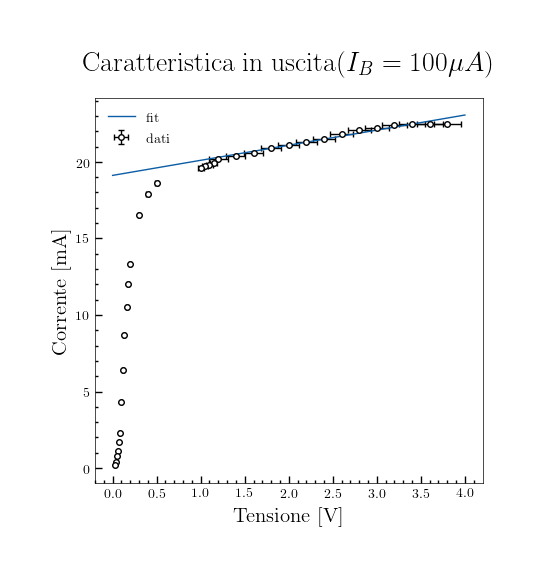
\includegraphics[width = 9cm, height = 9cm]{ib100/grafico_transistor.png}
        \hspace{0.1cm}
        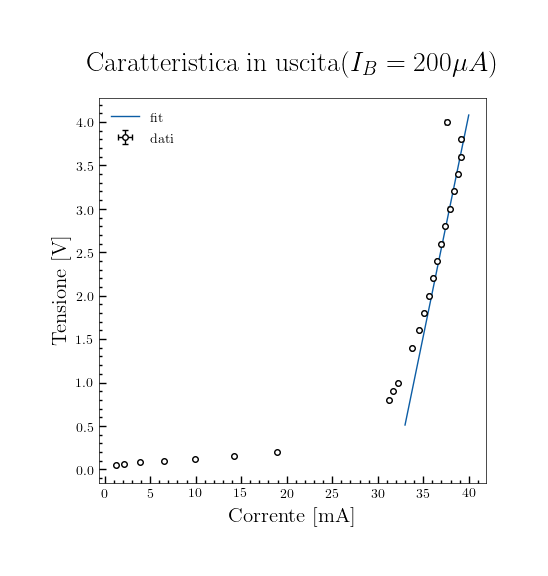
\includegraphics[width = 9cm, height = 9cm]{ib200/grafico_transistor.png}
    \end{center}
    \newpage
    Nonostante i valori di tensione e resistenza siano effettivamente negativi ne sono omessi i segni nelle tabelle e nei grafici.\\
    I dati misurati con corrente di base 10$\mu$A e 200$\mu$A sono:\\
    \begin{center}
        \begin{tabular}{|p{1cm}|p{1cm}|p{1cm}|p{1cm}|p{2cm}|}
            \hline
            \multicolumn{5}{|c|}{Corrente di base 100$\mu$A}\\
            \hline
            \textbf V[V] & $\delta$V[V] & I[mA] & $\delta$I[mA] & fondoscala$[V]$ \\
            \hline
            0.07 & 0.003 & 0.01 & 0.0004\\
0.08 & 0.003 & 0.01 & 0.0004\\
0.1 & 0.004 & 0.02 & 0.0005\\
0.12 & 0.004 & 0.04 & 0.0007\\
0.14 & 0.005 & 0.07 & 0.001\\
0.16 & 0.008 & 0.1 & 0.004\\
0.18 & 0.009 & 0.16 & 0.005\\
0.2 & 0.009 & 0.24 & 0.005\\
0.24 & 0.01 & 0.53 & 0.008\\
0.26 & 0.01 & 0.73 & 0.01\\
0.28 & 0.02 & 1.07 & 0.04\\
0.29 & 0.02 & 1.26 & 0.04\\
0.3 & 0.02 & 1.48 & 0.04\\
0.31 & 0.02 & 1.74 & 0.05\\
0.32 & 0.02 & 2.03 & 0.05\\

            \hline      
        \end{tabular}
        \hspace{1cm}
        \begin{tabular}{|p{1cm}|p{1cm}|p{1cm}|p{1cm}|p{2cm}|}
            \hline
            \multicolumn{5}{|c|}{Corrente di base 200$\mu$A}\\
            \hline
            \textbf V[V] & $\delta$V[V] & I[mA] & $\delta$I[mA]  & fondoscala$[V]$ \\
            \hline
            0.07 & 0.003 & 0.01 & 0.0004\\
0.08 & 0.003 & 0.01 & 0.0004\\
0.1 & 0.004 & 0.02 & 0.0005\\
0.12 & 0.004 & 0.04 & 0.0007\\
0.14 & 0.005 & 0.07 & 0.001\\
0.16 & 0.008 & 0.1 & 0.004\\
0.18 & 0.009 & 0.16 & 0.005\\
0.2 & 0.009 & 0.24 & 0.005\\
0.24 & 0.01 & 0.53 & 0.008\\
0.26 & 0.01 & 0.73 & 0.01\\
0.28 & 0.02 & 1.07 & 0.04\\
0.29 & 0.02 & 1.26 & 0.04\\
0.3 & 0.02 & 1.48 & 0.04\\
0.31 & 0.02 & 1.74 & 0.05\\
0.32 & 0.02 & 2.03 & 0.05\\

            \hline
        \end{tabular}
    \end{center}
    \hfill \\
    I risultati finali sono:\\
    \begin{center}
        \begin{tabular}{|p{2cm}|p{1cm}|p{3cm}|}
            \hline
            \multirow{3}{*}{$I_B = 100mA$} & $a_1$ & $(19.1 \pm 0.1)V$ \\
                                        & $b_1$ & $(0.99 \pm 0.05) k \Omega$\\
                                        & $g_1$ & $(1.01 \pm 0.05) m \mho $\\
            \hline
            \multirow{3}{*}{$I_B = 200mA$} & $a_2$ & $(26.62 \pm 0.05)V$ \\
                                        & $b_2$ & $(2.76 \pm 0.03) k \Omega$\\
                                        & $g_2$ & $(0.362 \pm 0.004) m \mho $ \\
            \hline
            \multicolumn{2}{|c|}{$\beta(-3V)$} & $157\pm9$ \\
            \hline
        \end{tabular}
    \end{center}
    \hfill \\
    Tali risultati sono stati ottenuti tramite un fit lineare pesato sugli errori dovuti all'oscilloscopio nel range di linearità delle due caratteristiche,
    dove le $a_i$ indicano le intercette, le $b_i$ le pendenze e le $g_i$ gli inversi delle pendenze e $\beta$ infine è il guadagno di corrente al variare
    della corrente di base per un $V_{CE} = -3V$.
\end{document}